\documentclass[10pt]{article}

\usepackage{fancyhdr}
\usepackage{graphicx}
\usepackage{ctex}
\usepackage[colorlinks,linkcolor=black]{hyperref}
\usepackage{xcolor}
\usepackage{listings}
\usepackage{geometry}


\lstset{
    numbers=left, 
    numberstyle= \tiny, 
    keywordstyle= \color{ blue!70},
    commentstyle= \color{red!50!green!50!blue!50}, 
    frame=shadowbox, % 阴影效果
    rulesepcolor= \color{ red!20!green!20!blue!20} ,
    escapeinside=``, % 英文分号中可写入中文
    xleftmargin=2em,xrightmargin=2em, aboveskip=1em,
    framexleftmargin=2em
} 


\newcommand\figcaption{\def\@captype{figure}\caption}
\newcommand\tabcaption{\def\@captype{table}\caption}


\pagestyle{fancy}
\lhead{《并行计算》实验报告}
\rhead{严愉程}

\makeatletter % 设置双线页眉
\def\headrule{{\if@fancyplain\let\headrulewidth\plainheadrulewidth\fi%
\hrule\@height 1.0pt \@width\headwidth\vskip1pt%上面线为1pt粗
%\hrule\@height 0.5pt\@width\headwidth  %下面0.5pt粗
\vskip-2\headrulewidth\vskip-1pt}      %两条线的距离1pt
\vspace{2mm}}     %双线与下面正文之间的垂直间距
\makeatother

% 版面布局控制
\baselineskip=15pt % 控制行距
\textheight 225mm  % 整个页面版芯的高度
\oddsidemargin 5.6mm
\evensidemargin 5.6mm
\parindent=2\ccwd  % 首行缩进的长度
\topmargin -5mm

\begin{document}

\begin{titlepage}
    \heiti
    \vspace*{64pt}
    \begin{center}
        \fontsize{56pt}{0} 西北工业大学\\
        \vspace*{36pt}
        \fontsize{48pt}{0}{实\quad 验\quad 报\quad 告}\\
        \vspace*{48pt}
        \LARGE(2020\~{}2021学年 秋季学期)\\
        \vspace*{48pt}
    
        \LARGE 课程名称\ \ \ \underline{\makebox[140pt]{《并行计算》}}\\
        \vspace*{72pt}
    
        \Large 姓名\ \ \underline{\makebox[108pt]{严愉程}}\\
        \Large 学号\ \ \underline{\makebox[108pt]{2017300138}}\\
        \Large 学院\ \ \underline{\makebox[108pt]{教育实验学院}}\\
        \Large 班级\ \ \underline{\makebox[108pt]{HC001706}}\\
        \Large 专业\ \ \underline{\makebox[108pt]{计算机科学与技术}}\\
    \end{center}
\end{titlepage}

\tableofcontents

\title{\bf\Large 《并行计算》实验报告}
\date{2020/12/30}
\author{\small 严愉程}
\maketitle

\thispagestyle{fancy}

\section{实验内容}

1.熟悉MPI编程环境,掌握MPI编程基本函数及MPI的相关通信函数用法,掌握MPI的主从模式及对等模式编程;

2.熟悉OpenMP编程环境,初步掌握基于OpenMP的多线程应用程序开发,掌握OpenMP相关函数以及数据作用域机制、多线程同步机制等。 

\section{实验环境}
ubuntu18.04,inteli7-7700HK 4核8线程,gcc8.2,OpenMPI 4.2.0。使用CMake构建。

\section{实验内容}
分别进行以下实验:1.用Monte-Carlo随机积分算法估算$\pi$值的并行算法;2.Floyd算法的并行化;3.N皇后问题并行算法

\subsection{Monte-Carlo随机积分算法估算$\pi$值的并行算法}

\subsubsection{算法原理}



\subsubsection{实验步骤}

\subsubsection{运行结果}

\subsubsection{算法分析}
分析不同n值、P值以及不同有序度时算法的运行时间,进行算法并行性能和可扩展性分析。(*)

\subsection{Floyd并行算法}

\subsubsection{算法原理}

\subsubsection{实验步骤}

第一版的算法,在通讯的手段上比较粗糙,随着最外层变量k的迭代过程中,每一次矩阵mat[][]更新都进行一次矩阵的同步,即每个线程都广播一次自己管辖的矩阵区域,如图\ref{floyd代码第一版的运行结果}。在$mat_size=4000$的节点数下,多线程的运行时间和单线程的差不多,虽然能够得出正确的结果,但加速比不理想。

\begin{figure}[htbp]
    \centering
    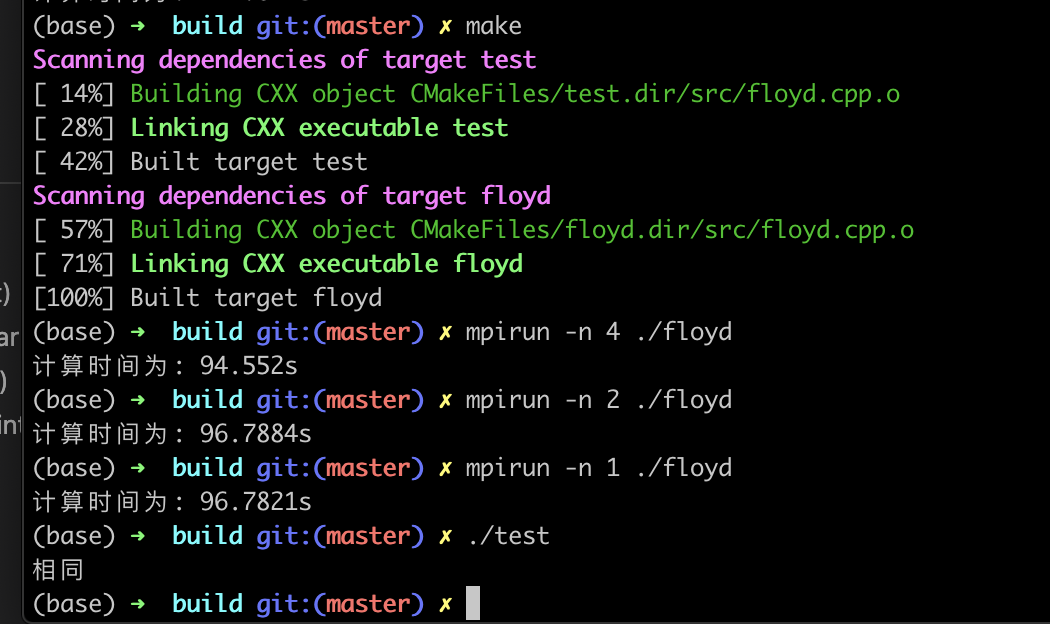
\includegraphics[width=.6\textwidth]{assets/floyd命令行运行界面.png}
    \caption{floyd代码第一版的运行结果}
    \label{floyd代码第一版的运行结果}
\end{figure}

考虑从通信量上的进行优化。在操作$mat[i][j] = \min(mat[i][k] + mat[k][j])$中,最外层循环k迭代的时候,$mat[i][k]$的数据永远在本线程管辖的区域内,不需要同步。而$mat[k][j]$会随着k的迭代,出现其他线程管辖的区域或者本线程管辖的区域是不确定的。

所以每次k迭代的时候,各个线程需要的是k行数据,迭代k行之前要广播k行。

需要注意的是,每次迭代的时候,实际上每个线程管辖的区域都更新了,最后还需要把这些更新进行同步,因为题目要求的是线程依次按照顺序分别写入,就不需要进行同步(在多节点的机器上应该不能做这种写入操作)。

改进之后的运行结果如图\ref{floyd优化版命令行运行结果}所示。

\begin{figure}[htbp]
    \centering
    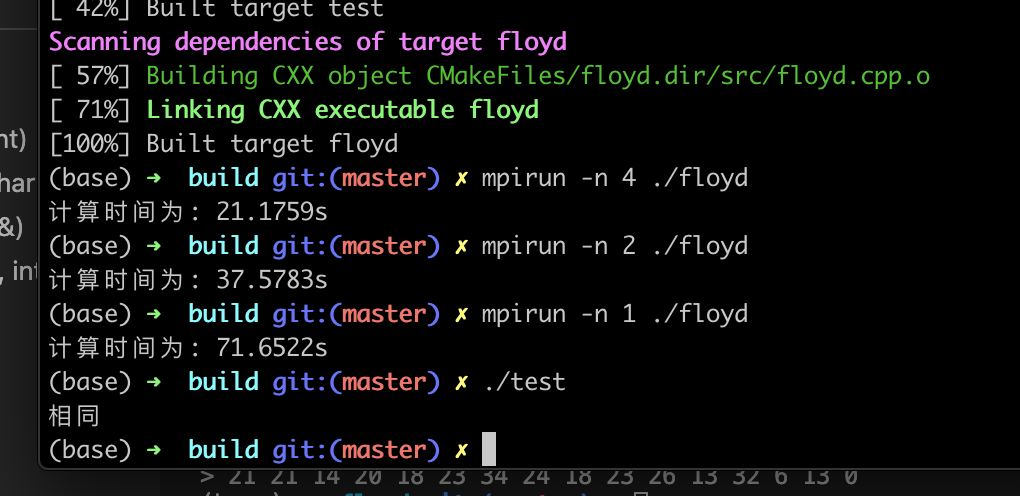
\includegraphics[width=.6\textwidth]{assets/floyd第二版命令行运行结果.png}
    \caption{floyd优化版命令行运行结果}
    \label{floyd优化版命令行运行结果}
\end{figure}



\subsubsection{运行结果}


\begin{table}[htbp]
    \centering
    \caption{floyd运行结果}
        \begin{tabular}{c|c|c|c}
        \hline
        矩阵的大小 & 线程数为1 & 线程数为2 & 线程数为4 \\
        \hline
        4000 & 71.6522s & 37.5783s & 21.1759s \\
        2000 & 9.36538s & 5.47045s & 3.69849s \\
        \hline
        \end{tabular}
    \label{label}
\end{table}

\subsubsection{算法分析}
分析不同n值、P值以及不同有序度时算法的运行时间,进行算法并行性能和可扩展性分析。(*)

\subsection{N皇后问题并行算法}

\subsubsection{算法原理}

\subsubsection{运行结果}

\subsubsection{算法分析}
分析不同n值、P值以及不同有序度时算法的运行时间,进行算法并行性能和可扩展性分析。(*)

\section{实验总结}



\end{document}

